\section{Cover decidability}
\label{sec:cover-decidability}

This section is devoted to proving the main result of this paper:

\begin{restatable}{theorem}{decidablecover}
\COVER for \BNRA{}s is decidable. Moreover, the problem is $\Fcomplexity{\omega^\omega}$-complete.
\end{restatable}

Thanks to Proposition~\ref{prop:loc-eq-test-elimination}, we may suppose that our protocols have no "local equality tests" (the complexity class $\Fomegaomega$ being stable by exponential reduction). 

The intuition of our decidability procedure is as follows. 
Consider a given run and a given agent $a$ that covers some state $q$. We are interested in what the agent needs from other agents to cover $q$. The agent $a$ might need to receive a sequence $w \in \messages^*$ of messages that all have the same value, so that it stores the value of the first such message then tests equality with the stored value upon reception of following messages. 
From the other agents' perspective, this means that someone (or several agents) are required to broadcast $w$ with the same value in every broadcast. We later call such a request a \emph{"boss specification"}.  
Moreover, the agent $a$ might first broadcast messages with some value $\aval$ that it had initially and require to receive from other agents messages with this same value $\aval$. 
From the other agent's perspective, this means that someone, after receiving sequence of messages $w$ all with the same value $\aval$, is required to broadcast a given message $\amessage$ with value $\aval$. We later call such a request a \emph{"follower specification"}.

The two roles identified previously are the key to the decidability procedure. While, in the original run, it could be that some agent plays several such roles\lu{it would be nice to have such an example in the execution example and cite it there}, we will in fact show, thanks to the copycat principle, that one might consider that each agent only plays one such role. We will use what we will name an "unfolding tree" as a way to list all "roles" needed for a local run to happen, and, in the same time, to verify that each of this "role" can be carried out.

Hence, an interesting unfolding tree is an "unfolding tree" with root a local run covering the state to cover $q_f$.
%We will define an "unfolding tree" of a local run where each node provides a witness that a given "role" can be carried out. 
We will then provide bounds on the size of the "unfolding tree" that we have to consider, and conclude that a decidability procedure can simply guess such an "unfolding tree". 

We will proceed as follows. In Section~\ref{sec:decidability-defs}, we introduce several usefuls notions. In Section~\ref{sec:decidability-tree-unfoldings}, we define the notion of "unfolding tree". In Section~\ref{sec:decidability-shortening-branches}, we provide useful arguments towards shortening branches of a tree. In Section~\ref{sec:local-bounds}, we provide useful arguments towards bounding the size of a given node of the tree. In Section~\ref{sec:tree-bounds}, we bound the overall size of the tree. In Section~\ref{sec:decidability-end}, we conclude by proving our decidability procedure. 


\subsection{Useful definitions}
\label{sec:decidability-defs}

We first need to define what is a "local run". A "local run" may be understood as the projection of a "run" onto a given agent. Among with "local runs", we define "local configurations" and "local steps".  When a "local step" describes the broadcast of a message we name it an "internal step", whereas when it describes a reception of a message with a certain value, we name it an "reception step". We also define a "trace" of a "local run" as the sequence of message types broadcast and received (and the received value when it is a reception) in the "local run".
	
\AP A ""local configuration"" is a pair $(q, \localdata) \in Q \times \nats^r$.  
\AP An ""internal step"" from $(q,\localdata)$ to $(q',\localdata')$ with transition $\atrans \in \transitions$, denoted $(q,\localdata) \intstep{\atrans} (q',\localdata')$, is defined when $\localdata = \localdata'$, and $\atrans =(q, \alpha, q')$ is either a "broadcast" or a "local test" and if it is "local test" on register $i$ and $j$, $\localdata(i) \ne \localdata(j)$.  
\AP A ""reception step"" from $(q,\localdata)$ to $(q',\localdata')$ with transition $\atrans \in \transitions$ and value $\aval \in \nats$, denoted $(q,\localdata) \extbr{\atrans}{\aval} (q',\localdata')$, is defined when $\atrans$ is of the form $(q,\rec{m}{j}{\anact},q')$ with $\localdata(j') = \localdata'(j')$ for all $j' \neq j$ and one of the following cases holds:
	
	\begin{minipage}[t]{6cm}
		\begin{itemize}
			\item $\anact = \quotemarks{\dummyact}$ 
			and $\localdata(j) = \localdata'(j)$
			\item $\anact = \quotemarks{\enregact}$ and $\localdata'(j) = v$
		\end{itemize}
	\end{minipage}
	\begin{minipage}[t]{6cm}
		\begin{itemize}
			\item $\anact = \quotemarks{\eqtestact}$ and $\localdata(j) = \localdata'(j)= v$
			\item $\anact = \quotemarks{\diseqtestact}$ and $\localdata(j) = \localdata'(j) \ne v$.
		\end{itemize}
	\end{minipage}
	

	%Said otherwise, $(q,\localdata) \extbr{\atrans}{\aval} (q',\localdata')$ when an agent in $(q,\localdata)$ may perform $\atrans$ upon receiving a message of type $\amessage$ and of value $\aval$.
	\AP A ""local step"" $(q,\localdata) \step{} (q',\localdata')$ is either an "reception step" or an "internal step". 
	\AP A ""local run"" is a sequence $\localrun$ of "local steps" $(q_0, \nu_0) \step{\locallabel_1} (q_1, \nu_1) \step{\locallabel_2} \cdots \step{\locallabel_k} (q_k, \nu_k)$ where, for all $i$, $\locallabel_i \in \set{\extlabel{\atrans}{\aval} \mid \atrans \in \transitions, \aval \in \nats} \cup \set{\intlabel{\atrans} \mid \atrans \in \transitions}$. 
	
	\AP A ""trace"" is a sequence in $(\set{\extlabel{\atrans}{\aval} \mid \atrans \in \transitions, \aval \in \nats} \cup \set{\intlabel{\atrans} \mid \atrans \in \transitions})^*$. The ""trace"" of a "local run" $\localrun$ is the "trace" $\trace{\localrun}$ containing the message types and values that $\localrun$ receives and broadcasts. Given a "trace" $\atrace$, we write $(q,\localdata) \step{\tau} (q',\localdata')$ to express that there exists a "local run" of "trace" $\atrace$ from $(q,\localdata)$ to $(q',\localdata')$. %peut-être qu'on peut mettre une partie de ça en annexe au niveau de la preuve du lemme tower

	

	Finally, we define the "input" and "output" of a "local run" $\localrun$: the "input", denoted by $\Input{\localrun} \in (\messages \times \nats)^*$, is the sequence containing messages types and values of its "reception steps". The output, denoted by $\Output{\localrun} \in (\messages \times \nats)^*$, is the sequence of messages types and values broadcast made in the "local run". The $\val$-input $\vinput{\aval}{\localrun} $ (resp. $\val$-output $\voutput{\aval}{\localrun}$) is the sequence containing message types of the "reception steps" (resp. the internal broadcasts steps) with value $\val$ made in $\localrun$. Formally, $\vinput{\aval}{\localrun}$ (resp. $\voutput{\aval}{\localrun}$) is the word $m_0 \cdots m_{\ell} \in \messages^*$ such that $(m_0, \aval) \cdots (m_{\ell}, \aval)$ is the projection of $\Input{\localrun}$ (resp. $\Output{\localrun}$) on $\messages \times \set{\aval}$. 
	\nicoin{faire le point sur ce qui peut aller en annexe là-dedans}
%	The ""input"" of a "local run" $\localrun$ is the sequence $\Input{\localrun} \in (\messages \times \nats)^*$ containing messages types and values of its "reception steps".
%	Similarly, its ""output"", which we denote by $\Output{\localrun} \in (\messages \times \nats)^*$, is the sequence of messages of (internal) broadcast steps made in $\localrun$.
%	Given a value $v \in \nats $, the $v$-input $\vinput{\aval}{\localrun} $(resp. the $v$-output $\voutput{\aval}{\localrun}$) of $\localrun$ is defined as the sequence of messages of $\Input{\localrun}$ (resp. $\Output{\localrun}$) that have value $\aval$. Formally, $\vinput{\aval}{\localrun}$ is the word $m_0 \cdots m_{\ell} \in \messages^*$ such that $(m_0, \aval) \cdots (m_{\ell}, \aval)$ is the projection of $\Input{\localrun}$ on $\messages \times \set{\aval}$. 
%	


\subsection{Unfolding trees}
\label{sec:decidability-tree-unfoldings}




\luin{le paragraphe ci dessous devra etre concisé }

Recall that the "unfolding trees" of interest should be rooted with a "local run" covering the state $q_f$. It should then, gives a list of "roles" to be carried out and verify if this is possible. Earlier, we mentionned two types of "roles": "boss specification" and "follower specification".
Before giving the defintion of the "unfolding trees", we should explain exactly what are their and how do the two roles fit in the tree.


Let $\localrun$ be the "local run" of an agent $a$, for $a$ to be able to perform its "local run" it may need to receive some sequences of messages among with some values. Each of this reception leads to an action (it might be a dummy action) on one of $a$'s registers.
From the "copycat principle", the challenging part is actually to keep track of messages which can be sent with the same value\lu{il faudrait que l'exemple générique illustre ça et le citer ici}. Take one moment in the local run of $a$ where the agent needs to receive a sequence of message $m_1, \dots m_k$ among with a value $\val$ and test its equality with one of its register $r$. We distinguish two possible situations for which $a$ can take the sequence of transitions: (i) agent $a$ stored value $\val$ in register $r$ earlier, (ii) value $\val$ is the initial value of register $r$. In case (i), we need to verify that some agents are able to send the sequence $m_1 \dots m_k$ with the same value. Agent $a$ does not need to intervene in this "role" as it is not the initial value of its register $r$. Note that if the value is the initial value of another register of $a$, then we can duplicate $a$ so the duty of propagating this initial value $\val$ is not let to agent $a$. This way, a "boss specification" can be described with a word of messages (here $m_1 \dots m_k$). This shall be read as:
\begin{center}
	The role of a set of agents with "boss specification" $w$ is to send the sequence of message $w$ with the same value.
\end{center}

Assume now we are in situation (ii). The only way for $a$ to receive some message among with value $\val$ is if some other agents \emph{repeated} the value after storing it (because $a$ is the only holder of value $v$ in the first place). As a consequence, agent $a$ necessarily broadcast some messages among with its value of register $r$. Name $w_0$ the sequence of messages agent $a$ broadcast with its register $r$ before receiving message $m_1$ (with value $\val$), then we need to check that some agent is able to send the message $m_1$ after receiving a subword of $w_0$, each message with value $\val$. Note that, as any number of agents can receive the sequence $w_0$, any number of agents can send the message $m_1$. This might not be of interest for agent $a$ but this will be for the agent which shall send $m_2$ with value $\val$ to agent $a$. Indeed, it is still left to check that some agents can send message $m_2$ with value $\val$, message $m_3$ with value $\val$ etc...\\
If agent $a$ broadcasts new messages with its register $r$ after receiving $m_1$, this should be taken into consideration when checking that an agent can carry out the role of sending $m_2$. Note $w_1$ the sequence of messages agent $a$ broadcast with its register $r$ after receiving $m_1$ and before receiving message $m_2$ (with value $\val$). Now, to send message $m_2$, an agent might have received any subword of $w_0$, and then, a word $w'_1$ where $w'_1$ is any subword of $w_1$ and some $m_1$ might have been inserted anywhere in the word. This comes from the unbounded number of agents now able to send $m_1$ with value $\val$.


We can repeat the argument to $m_3$ and so on: note $w_2$ the sequence of messages broadcast by agent $a$ with register $r$ between receiving $m_2$ and $m_3$, an agent whose role is to send message $m_3$ might have received any sequence $w'_0\cdot w'_1 \cdot w'_2$ where: $w'_0$ is any subword of $w_0$, $w'_1$ is any subword of $w_1$ where some $m_1$ were inserted, and $w'_2$ is any subword of $w_2$ where some $m_1$ and $m_2$ were inserted. A "follower specification" in that case should be the word $w'_0 \cdot w'_1 \cdot w'_2$ among with message $m_3$, and should be read as:
\begin{center}
		{The role of a set of agents with "follower specification" $w, m$ is to send message $m$ with a value, after receiving the sequence of messages $w$ with the same value. In addition, this value shall not be any of the initial values of the agent}.
\end{center}
Even in this case we write a set of agents rather than an agent because this agent might need some other agents in order to perform its task.
%
%
%Consider an agent $a$ that initially has value $\aval$ in one of its registers. After broadcasting some word $w$ with value $\aval$, $a$ may need some other agent to broadcast $\amessage_1$ with value $\aval$. An agent doing so did not have $\aval$ initially, hence it may be cloned at will: we are able to send $\amessage_1$ with value $\aval$ as many times as we want. Then, if $a$, after broadcasting $w_2$ with value $\aval$, must receive a message $\amessage_2$ with value $\aval$, then the agent broadcasting $\amessage_2$ may receive with value $\aval$ a word of the form $w_1 \cdot w_2'$ where $w_2'$ is $w_2$ where some $\amessage_1$ were inserted. Similarly, if $a$ then needs $\amessage_3$ with value $\aval$ after broadcasting $w_3$, then an agent playing that role may beforehand receive with value $\aval$ a word of the form $w_1 \cdot w_2'' \cdot w_3''$ where $w_2''$ is $w_2$ where some $\amessage_1$ were inserted, and $w_3''$ is $w_3$ where some $\amessage_2$ and $\amessage_3$ were inserted. 


We may now formally define our unfolding trees which abstractly represent executions. 
\AP An ""unfolding tree"" $\tree$ over $\prot$ is
a finite tree where each node $\node$ has three labels:
\begin{itemize}
	\item The first one is a local run of $\prot$, written $\localrunlabel{\node}$. 
	
	\item The second one is a value, written $\valuelabel{\node}$.
	
	\item The third one is a ""specification"" $\speclabel{\node}$, which is either a word $\bosslabel{\node} \in \messages^*$ (""boss specification"") or a pair $(\followlabelword{\node}, \followlabelmessage{\node}) \in \messages^* \times \messages$ (""follower specification""). In the first case we say that the node is a ""boss node"", otherwise it is a ""follower node"".
\end{itemize} 


For a ""follower node"" $\node$, we will need to represents the possible sequences for $\followlabelword{\node}$ depending on the available messages. Remember that for the "local run" $\localrun$ of agent $a$ earlier, there was an infinite number of possible sequences $w_0' \cdot w_1' \cdot w_2'$ because any number of $m_1$ and $m_2$ could be added to the subwords of $w_2$. We find a way to describe all the possible sequence from $(w_0, m_1, w_1, m_2, w_2)$ in the following way:

A ""decomposition"" is a tuple $\decsymb = (w_0, m_1, \ldots, m_\ell, w_\ell)$ with $w_0, \ldots, w_\ell \in \messages^*$, and $m_1, \cdots, m_\ell \in \messages$, with $m_i \neq m_j$ for all $i\neq j$. In particular we have $\ell \leq \size{\messages}$. 

We say that $w \in \messages^*$ ""admits decomposition"" $\decsymb = (w_0, m_1, \ldots, m_\ell, w_\ell)$ if $w \subword w'_0 w'_1 \cdots w'_\ell$ where for all $j$, $w'_j$ can be obtained from $w_j$ by adding letters from $\set{m_1, \ldots, m_{j-1}}$.
We denote by $\langdec{\decsymb}$ the language of words that admit decomposition $\decsymb$. 

As we argued earlier, the set of sequences $w_0' \cdot w_1' \cdot w_2'$ is exaclty the language $\langdec{\decsymb}$ for $\decsymb = (w_0, m_1, w_1, m_2, w_2)$.

For $\aval$ appearing in a "local run", $\aval$ is ""initial"" if its appears in $u$'s first "local configuration", and ""non-initial"" otherwise. \nicoin{a enlever?}


We now state some conditions on the links between a node and its children. Intuitively, the desired property is the following: 

Let $\node$ a node of $\tree$. 
The conditions expressed below state two things. First, that $\node$ is a witness that its "specification" is carried out. Second, that the "specifications" of its children are witnesses that messages received in the "local run" $\localrunlabel{\node}$ can be broadcast by other agents (\ref{item:condition1_}). It is formalized as follows.
\begin{enumerate}[{Condition} (i)]
	\item \label{item:condition1_non_initial_value} For every non-initial value $\aval \ne \valuelabel{\node}$ of $\localrun$, $\node$ has a child $\node'$ which is a "boss node" such that $\vinput{\aval}{\localrun}$ is a subword of $\bosslabel{\node'}$.
	
	\item \label{item:condition2_initial_value} For every initial value $\aval$ of $\localrun$, there is a "decomposition" $\decsymb = (w_0, m_1, w_1, \ldots, m_{\ell}, w_{\ell})$ s.t.:
	\begin{itemize}
		\item $\localrun$ may be split into successive "local runs" $\localrun_0, \dots, \localrun_{\ell}$ where, for all $i \in \nset{1}{\ell}$, $w_i \subword \voutput{\aval}{\localrun_i}$ and $\vinput{\aval}{\localrun_i} \in \set{m_1, \dots, m_{i-1}}^*$
		\item for all $i \in [1,\ell]$, $\node$ has a child $\node_i$ which is a "follower node" such that $\followlabelmessage{\node_i} = m_i$ and $\followlabelword{\node_i} \in\langdec{\decsymb_i}$ where $\decsymb_i = (w_0, m_1, w_1, \ldots, m_{i-1}, w_{i-1})$.	\end{itemize}
	
	\item \label{item:condition3_follower_node} If $\node$ is a "follower node" then $\aval$ is not an initial value of $\localrun$, $\vinput{\aval}{\localrun} = \followlabelword{\node}$ and 
	$\voutput{\aval}{\localrun}$ contains $\followlabelmessage{\node}$.

	\item \label{item:condition4_boss_node} If $\node$ is a "boss node", there $\valuelabel{\node}$ is an "initial value" of $\localrunlabel{\node}$ and the associated "decomposition" $\decsymb$ of \ref{item:condition2_initial_value} satisfies that $\bosslabel{\node} \in \langdec{\decsymb}$.
\end{enumerate}

There is a strong connection between runs of $\prot$ and "unfolding trees". In fact, the following proposition expresses that \COVER may be expressed as the existence of an "unfolding tree". 
The proof can be found in Appendix~\ref{app:trees-sound-complete}.


\begin{restatable}{proposition}{treessoundcomplete}
\label{prop:trees-sound-complete}
Let $(\prot,q_f)$ an instance of $\COVER$. $(\prot,q_f)$ is positive if and only if there exists an "unfolding tree" $\tree$ of $\prot$ such that the local run at the root of $\tree$ covers $q_f$.
\end{restatable}



\subsection{Shortening branches}
\label{sec:decidability-shortening-branches}

\begin{restatable}{lemma}{lemIncreasingBosses}
	\label{lem:increasing-bosses}
	Let $\tree$ be a "unfolding tree" satisfying a specification $\spec$.
	Let $\node, \node'$ be two "boss nodes" of $\tree$.
	If $\node$ is an ancestor of $\node'$ and $\bosslabel{\node}$ is a subword of $\bosslabel{\node'}$ then there exists a smaller "unfolding tree" satisfying $\spec$.  
\end{restatable}

\begin{restatable}{lemma}{lemIncreasingFollowers}
	\label{lem:increasing-followers}
	Let $\tree$ be a "unfolding tree" satisfying a specification $\spec$.
	Let $\node, \node'$ be two "follower nodes" of $\tree$.
	If $\node$ is an ancestor of $\node'$, $\followlabelword{\node'} \subword \followlabelword{\node}$ and $\followlabelmessage{\node'}=\followlabelmessage{\node}$ then there exists a smaller "unfolding tree" satisfying $\spec$. 
\end{restatable}


\subsection{Local bounds}
\label{sec:local-bounds}


\begin{figure}
	

	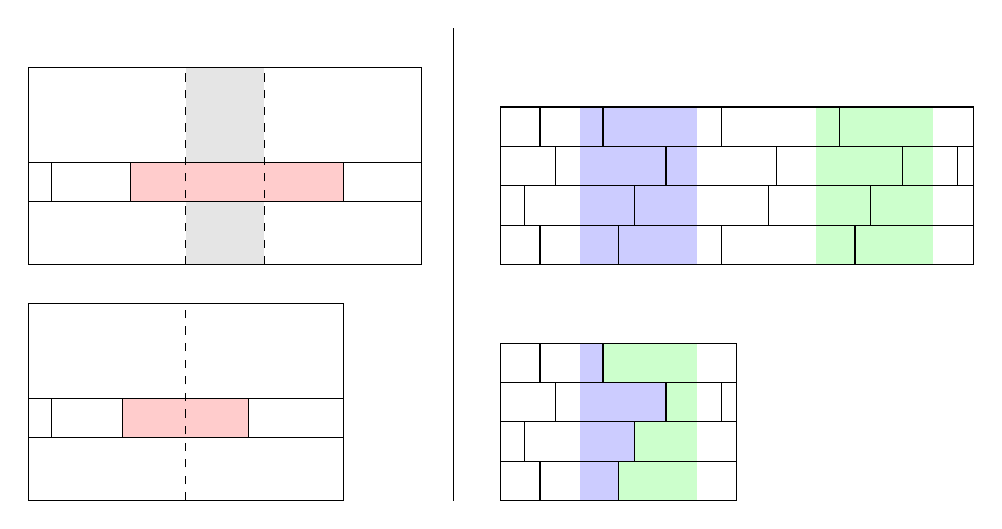
\begin{tikzpicture}
		\draw[white,fill=gray!20] (2,0) rectangle (3,0.8);
		\draw[white,fill=gray!20] (2,1.3) rectangle (3,2.5);
		
		\draw (0,0) rectangle (5,2.5);
		
		\draw (0,0.8) rectangle (5,1.3);
		
		\draw (0,0.8) rectangle (0.3,1.3);
		\draw (0,0.8) rectangle (1.3,1.3);
		\draw[fill=red!20] (1.3,0.8) rectangle (4,1.3);
		
		\draw[dashed] (2,0) -- (2,2.5);
		\draw[dashed] (3,0) -- (3,2.5);
		
		
		
		\draw (0,-3) rectangle (4,-0.5);
		
		\draw (0,-2.2) rectangle (4,-1.7);
		
		\draw (0,-2.2) rectangle (0.3,-1.7);
		\draw (0.3,-2.2) rectangle (1.3,-1.7);
		\draw[fill=red!20] (1.2,-2.2) rectangle (2.8,-1.7);
		
		\draw[dashed] (2,-3) -- (2,-0.5);
		
		\draw (5.4,-3) -- (5.4,3);
		
		
		\draw[white,fill=blue!20] (7,0) rectangle (8.5,2);
		\draw[white,fill=green!20] (10,0) rectangle (11.5,2);
		
		\draw (6,0) rectangle (12,2);
		
		\draw (6,0) rectangle (12,0.5);
		\draw (6,0) rectangle (12,1);
		\draw (6,0) rectangle (12,1.5);
		
		\draw (6,0) rectangle (6.5,0.5);
		\draw (6,0) rectangle (7.5,0.5);
		\draw (6,0) rectangle (8.8,0.5);
		\draw (6,0) rectangle (10.5,0.5);
		
		\draw (6,0.5) rectangle (6.3,1);
		\draw (6,0.5) rectangle (7.7,1);
		\draw (6,0.5) rectangle (9.4,1);
		\draw (6,0.5) rectangle (10.7,1);
		
		\draw (6,1) rectangle (6.7,1.5);
		\draw (6,1) rectangle (8.1,1.5);
		\draw (6,1) rectangle (9.5,1.5);
		\draw (6,1) rectangle (11.1,1.5);
		\draw (6,1) rectangle (11.8,1.5);
		
		\draw (6,1.5) rectangle (6.5,2);
		\draw (6,1.5) rectangle (7.3,2);
		\draw (6,1.5) rectangle (8.8,2);
		\draw (6,1.5) rectangle (10.3,2);
		
		
		\draw[white, fill=blue!20] (7,-3) rectangle (7.5,-2.5);
		\draw[white,fill=blue!20] (7,-2.5) rectangle (7.7,-2);
		\draw[white,fill=blue!20] (7,-2) rectangle (8.1,-1.5);
		\draw[white,fill=blue!20] (7,-1.5) rectangle (7.3,-1);
		
		\draw[white,fill=green!20] (7.5,-3) rectangle (8.5,-2.5);
		\draw[white,fill=green!20] (7.7,-2.5) rectangle (8.5,-2);
		\draw[white,fill=green!20] (8.1,-2) rectangle (8.5,-1.5);
		\draw[white,fill=green!20] (7.3,-1.5) rectangle (8.5,-1);
		
		
		
		\draw (6,-3) rectangle (9,-2.5);
		\draw (6,-3) rectangle (9,-2);
		\draw (6,-3) rectangle (9,-1.5);
		\draw (6,-3) rectangle (9,-1);
		
		\draw (6,-3) rectangle (6.5,-2.5);
		\draw (6,-3) rectangle (7.5,-2.5);
		
		\draw (6,-2.5) rectangle (6.3,-2);
		\draw (6,-2.5) rectangle (7.7,-2);
		
		\draw (6,-2) rectangle (6.7,-1.5);
		\draw (6,-2) rectangle (8.1,-1.5);
		\draw (6,-2) rectangle (8.8,-1.5);
		
		\draw (6,-1.5) rectangle (6.5,-1);
		\draw (6,-1.5) rectangle (7.3,-1);
		
	\end{tikzpicture}


	\caption{Illustration of the proof of Lemma~\ref{lem:short-local-runs}. We represent local runs as above, where Lines correspond to registers, and vertical separations are times at which a $\enregact$ operation is performed on that register. If one register $i$ keeps the same value for a long enough time (on the left), we apply the induction hypothesis to shorten the projection of the run on the other registers. As the value of $i$ does not change, the resulting run is still valid. If all registers change values often, say every $M$ steps (on the right), then if the run is long enough we can find two identical sequences of transitions during which all values are renewed twice. We can then obtain a shorter run by glueing them together as in the picture. The colored rectangles in the shortened runs correspond to fresh values that we introduce to make sure that all local disequality tests succeed.}
\end{figure}
\begin{restatable}{lemma}{lemShortLocalRuns}
	\label{lem:short-local-runs}
	There exists a primitive recursive function $\towerfun(n) (\regnum)$ such that, for every protocol $\prot$ with $r$ registers per process, for every "local run" $\localrun: (q, \localdata) \step{*} (q', \localdata')$ in $\prot$, for every $V \subseteq \nats$ finite that contains every message value appearing in $\localrun$, there exists $\localrun': (q, \localdata) \step{*} (q', \localdata')$\corto{uniformiser la notation} such that $\length{\localrun'} \leq \towerfun(\size{\prot})(r)$ and:
	\begin{enumerate}
		\item \label{item:shorterrun_anyvalue} for all $\aval' \in \nats$, there exists $\aval \in \nats$ such that $\vinput{\aval'}{\localrun'}$ is a subword of $\vinput{\aval}{\localrun}$,
		\item \label{item:shorterrun_oldvalues} for all $\aval \in V$, $\vinput{\aval}{\localrun'}$ is a subword of $\vinput{\aval}{\localrun}$. 
		% \item by writing $V := \nats \setminus \set{\localdata_i(k) \mid k \in \nset{1}{\regnum}}$, for every $\aval' \in V$, there exists $\aval \in V$ such that $\vinput{\aval'}{\localrun'}$ is a subword of $\vinput{\aval}{\localrun}$.
	\end{enumerate}
		%  with an "input" $I$.
% 	Let $u_1, u_2, u_3$ be such that $u=u_1u_2u_3$.
% 	If $\size{u_2} > TOWER$, then there exists $u'_2$ with $|u_2'| \leq \towerfun(\prot)$ such that $u_1u'_2u_3$ is a local run of $\prot$ with smaller "input" than $u$. 
\end{restatable}

\begin{remark}
	The tower bound of Lemma~\ref{lem:short-local-runs} is tight, in the sense that some local runs may need to have length a tower of exponentials of linear height in the number of registers.
	It also holds for pushdown automata, as the .
	\cortoin{To formalize}
\end{remark}


\begin{restatable}{lemma}{lemShortRunOutput}
	\label{lem:short-run-for-output}
	For every protocol $\prot$ with $r$ registers per process, for every $w_{in} \in (\messages\times \nats)^*$, if there exists a "local run" $\localrun: (q, \localdata) \step{*} (q', \localdata')$ in $\prot$ such that $w_{in} \subword \Output{\localrun}$, then for every $V \subseteq \nats$ finite that contains every message value appearing in $\localrun$, there exists $\localrun': (q, \localdata) \step{*} (q', \localdata')$ such that $\length{\localrun'} \leq (\towerfun(\size{\prot})(r)+1)\size{w_{in}}$, $w_{in} \subword \Output{\localrun'}$ and:
	
	\begin{enumerate}
		\item for all $\aval' \in \nats$, there exists $\aval \in \nats$ such that $\vinput{\aval'}{\localrun'}$ is a subword of $\vinput{\aval}{\localrun}$,
		\item for all $\aval \in V$, $\vinput{\aval}{\localrun'}$ is a subword of $\vinput{\aval}{\localrun}$. 
	\end{enumerate}
\end{restatable}


\begin{restatable}{lemma}{lemBoundSuccessorHeight}
	\label{lem:bound-successor-height}
	Let $\prot$ be a "protocol" over $\regnum$ registers, let $\node$ be a node of a "unfolding tree" $\tree$ of minimal size labelled by $\prot$ satisfying a "boss specification" $w$.
	Let $\node_1, \ldots, \node_k$ be its "follower" children. If $\node$ is not the root of $\tree$ then let $\mu'$ be its father.
	We have the following properties:
	
	\begin{enumerate}
		\item $k \leq \size{\messages}r$ 
		
		\item The root of $\tree$ is a "boss node".
				
		\item  If $\node$ is a "boss node" then 
		\begin{itemize}
			\item If $\node$ is the root of $\tree$ then $\bosslabel{\node} = w$
			
			\item If $\node$ is not the root then $\size{\bosslabel{\node}} \leq \size{\localrunlabel{\node'}}$
			
			\item In both cases $\size{\localrunlabel{\node}} \leq (\towerfun(\size{\prot})(r) + 1)\Big[ \size{\bosslabel{\node}} + \sum_{i=1}^k \size{\followlabelword{\node_i}} \Big]$
		\end{itemize}
	
		\item If $\node$ is a "follower node" then 
		\begin{itemize}			
			\item $\size{\followlabelword{\node}} \leq \size{\localrunlabel{\node}}$
			
			\item $\size{\localrunlabel{\node}} \leq (\towerfun(\size{\prot})(r) +1)\Big[ 1 + \sum_{i=1}^k \size{\followlabelword{\node_i}} \Big]$
			
		\end{itemize}
	\end{enumerate}
\end{restatable}


\subsection{Tree bounds}
\label{sec:tree-bounds}

\begin{definition}
	We define the ""altitude"" of a node $\node$, written $\altitude{\node}$, in a "unfolding tree" recursively as follows:
	\begin{itemize}
		\item The altitude of the root is $0$
		
		\item The altitude of a "boss node" is the altitude of its father minus one
		
		\item The altitude of a "follower node" is the altitude of its father plus one.
	\end{itemize}
\end{definition}

\begin{restatable}{lemma}{lemBoundLengthHeightH}
	\label{lem:bound-length-at-height-h}
	Let $\prot$ be a protocol, let $\node$ be a node of a "unfolding tree" of minimal size labelled by $\prot$ satisfying a "boss specification" $w$.
	Let $\altmax$ be the maximal "altitude" in $\tau$, let $N = \size{w} + \size{\prot} +1$ and let $f_0 : \nats \to \nats$ be the function mapping each $n \in \nats$ to $f_0(n)=(N^2 (\towerfun(N)(N) + 1))^{n+1}$ 
	
	\begin{itemize}
		\item If $\node$ is a "boss node" then $\size{\bosslabel{\node}} \leq f_0(\altmax - \altitude{\node}-1)$ and $\size{\localrunlabel{\node}} \leq f_0(\altmax - \altitude{\node})$.
		
		\item If $\node$ is a "follower node" then $\size{\localrunlabel{\node}} \leq \size{\followlabelword{\node}} \leq  f_0(\altmax - \altitude{\node})$.
	\end{itemize} 
\end{restatable}

\begin{restatable}{lemma}{lemBoundMaxHeight}
	\label{lem:bound-max-height}
	There exists a function $f_1$ of the class $\Ffunction{\omega^{\size{\messages}}}$ such that for all "protocol" $\prot$, for all "unfolding tree" $\tree$ of minimal size labelled by $\prot$ satisfying a "boss specification" $w$, the maximal altitude of a node of $\tree$ is bounded by $f_1(\size{\prot} + \size{w}+1)$.
\end{restatable}


\begin{restatable}{lemma}{lemBoundMinHeight}
	\label{lem:bound-min-height}
	There exists a function $f_2$ of the class $\Ffunction{\omega^{\size{\messages}+1}}$ such that for all "protocol" $\prot$, for all "unfolding tree" $\tree$ of minimal size labelled by $\prot$ satisfying a "boss specification" $w$, the absolute value of the minimal "altitude" of a node of $\tree$ is bounded by $f_2(\size{\prot} + \size{w}+1)$.
\end{restatable}



\begin{corollary}
	\label{cor:bound-node-size}
	There exists a function $f_3$ of the class $\Ffunction{\omega^{\size{\messages}+1}}$\corto{corriger les M en M+1} such that for all "protocol" $\prot$, for all "unfolding tree" $\tree$ of minimal size labelled by $\prot$ satisfying a "boss specification" $w$, for all node $\node$ of $\tree$,
	
		\begin{itemize}
		\item $\size{\localrunlabel{\node}} \leq f_3(\size{\prot}+ \size{w})$
			
		\item If $\node$ is a "boss node" then $\size{\bosslabel{\node}} \leq f_3(\size{\prot}+ \size{w})$.
		
		\item If $\node$ is a "follower node" then $\size{\followlabelword{\node}} \leq f_3(\size{\prot}+ \size{w})$.
	\end{itemize} 
\end{corollary}

\ifproofs
\begin{proof}
	Consequence of Lemmas~\ref{lem:bound-length-at-height-h}, \ref{lem:bound-max-height} and \ref{lem:bound-min-height} as $\Ffunction{\omega^{\size{\messages}+1}}$ is closed by composition with elementary functions.
\end{proof}
\fi
\begin{restatable}{proposition}{PropBoundTreeSize}
	\label{prop:bound-tree-size}
	There exists a function $f_4$ of the class $\Ffunction{\omega^{\size{\messages}+1}}$ such that for all "protocol" $\prot$, for all "unfolding tree" $\tree$ of minimal size labelled by $\prot$ satisfying a "boss specification" $w$, the size of $\tree$ is bounded by $f_4(\size{\prot} + \size{w}+1)$.
\end{restatable}




\subsection{Decidability}
\label{sec:decidability-end}

\decidablecover*

\ifproofs
\begin{proof}
	The lower bound is given by the reduction from "lossy channel systems" reachability in Proposition~\ref{prop:reduction-LCS}.
	
	For the upper bound, let $\prot$ be a "protocol" with $\regnum \geq 1$ registers over messages $\messages$ and $q$ one of its states. We add a new message $m$ to $\messages$ and a new transition $\br{m}{1}$ from $q$ to itself broadcasting $m$. 
	Clearly the new "protocol" $\prot'$ satisfies the "boss specification" $m$ if and only if $q$ is coverable in $\prot$.
	
	By Lemmas~\ref{lem:run-to-tree} and \ref{lem:tree-to-run}, there is a run of $\prot'$ satisfying $m$ if and only if there is a "unfolding tree" satisfying $m$.
	By Lemma~\ref{prop:bound-tree-size}, there is such a "unfolding tree" if and only if there is one of size at most $f_4(\size{\prot}+2)$, where $f_4$ is a function of the class $\Ffunction{\omega^{\size{\messages}}}$.
	
	The last problem we have is that the size of a "unfolding tree" does not take into account the values used in it. This can be solved by noticing that the conditions in the definition of a "unfolding tree" and the condition to satisfy a "specification" still hold after applying an injective renaming to the values. 
	
	Suppose there exists $\tree$ a "unfolding tree" satisfying $m$, let $V$ be the set of values appearing in that tree. In a node $\node$ the values appearing are $\valuelabel{\node}$, the initial values of $\localrunlabel{\node}$ (there are $r$ such values), the non-initial values (at most $\size{\localrunlabel{\node}}$ as they all need to be received).
	Hence there are at most $\size{\localrunlabel{\node}} + r +1$ different values appearing in each node.
	In total there are thus at most $\sum_{\node \in \tree} \size{\localrunlabel{\node}} + r +1$ different values in $\tree$, which is less than $(r+2)\size{\tree}$.
	
	We can apply an injective renaming $V \to \nset{1}{(r+2)\size{\tree}}$ to the values to obtain another "unfolding tree" satisfying $m$ and whose values do not exceed $(r+2)\size{\tree}$.
	As a result, there exists a "unfolding tree" satisfying $m$ if and only if there is one of size at most $f_4(\size{\prot}+2)$ in which values do not exceed $f_4(\size{\prot}+2)$. A description of such a tree requires a space that is polynomial in its size.
	
	We can therefore bound the size of the description of such a "unfolding tree" by a function of $\Ffunction{\omega^{\size{\messages}}}$.
	An algorithm for the coverability problem thus consists in enumerating all trees labelled by local runs of $\prot$ of size at most $f_4(\size{\prot}+2)$ with values not exceeding $f_4(\size{\prot}+2)$, and accepting if and only if one of them satisfies the conditions to be a "unfolding tree" satisfying $m$.
	This can all be done in exponential time in $f_4(\size{\prot}+2)$, thus this algorithm terminates in time $f_5(\size{\prot})$ where $f_5$ is a function of $\Ffunction{\omega^{\size{\messages}}}$.
	
	The BNRA coverability problem is thus decidable in time $\Ffunction{\omega^\omega}$.
\end{proof}
\fi
